\section{Exponential and Logarithmic Functions}
We now present our main contribution in this paper: a general method to improve the general accuracy of the logarithm approximation given by Khattri in \cite{khattri_new_2009} for use in privacy-preserving calculation, provided that accuracy is only required for a specific range.

For this approximation, we assume we only require accurate results in the input range $x \in [0, 255]$. This reflects some potential applications such as in logarithm intensity transformations in image processing \cite{gonzalez_digital_2008}.

Since the approximation by Khattri is accurate for values of $x$ near zero, we can scale the approximation by a constant factor $\alpha$ by expressing $\log(1+x)$ as follows, similarly using the substitution $x=1/n$:
\begin{align*}
	\log{(1+x)} &= \log{\left(\frac{\alpha + \alpha x}{\alpha}\right)}\\
	&= \log{(\alpha + \alpha x)} - \log{\alpha}\\
	&= \log{\left(\alpha+\frac{\alpha}{n}\right)} - \log{\alpha}\\
	&= \log{\left(\frac{\alpha n + \alpha}{n}\right)} - \log{\alpha}\\
	&= \int_{n}^{\alpha n + \alpha}{\frac{1}{t}\diff t} - \log{\alpha}.
\end{align*}

Applying the five-point Gauss-Legendre quadrature rule to approximate $\int_{n}^{\alpha n + \alpha}{\frac{1}{x}\diff x}$ with $\alpha = 1/16$ using SageMath 8.3, we arrive at the approximation:
\begin{align}\label{eq:optimal_log_approximation}
	\begin{split}
		&\log(1+x) \\
		&=\frac{137x^5 + 26685x^4 + 617370x^3 - 6498630x^2 - 121239315x - 257804775}
		{30(x^5 + 405x^4 + 27210x^3 + 488810x^2 + 2536005x + 3122577)}\\
		&+ \log{16}
	\end{split}
\end{align}

We note that the approximation in equation \ref{eq:optimal_log_approximation} requires the value of $\log{16}$. This can be computed in the plaintext domain and added to an encrypted value using the properties of the Paillier cryptosystem. The remaining arithmetic operations in the approximation can be computed in the encrypted domain, using the protocols described in section \ref{sec:fp_operations}. Therefore, this approximation can be calculated in a privacy-preserving manner.

Figure \ref{fig:log_error_comparison} is a graph comparing the absolute error of the scaled approximation and the original approximation by Khattri given an input $x$. We can see that scaling the input by some constant factor $\alpha$ improves the accuracy of the closed-form approximation, although it requires that $\log \alpha$ be known.

\begin{figure}[!ht]
		\centering
		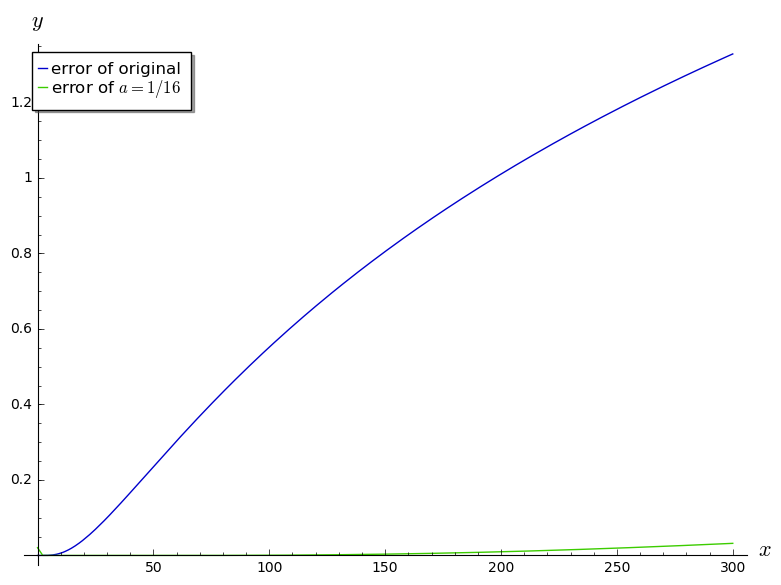
\includegraphics[width=.9\linewidth]{figures/log_error_comparison.png}
		\caption{Comparison of the absolute error between the original approximation in equation \ref{eq:standard_logarithm_quadrature} and the scaled approximation in equation \ref{eq:optimal_log_approximation}.}
		\label{fig:log_error_comparison}
\end{figure}

We now show how we used numerical methods to determine that a scaling factor of $\alpha = 1/16$ minimizes the maximum absolute error of the scaled approximation for $\log{(1+x)}$, within the range $x \in [0, 255]$.
Let the function $I(x,\alpha)$ be the function obtained by approximating $\int_{n}^{\alpha n + \alpha}{\frac{1}{x}\diff x}$ with five-point Gauss-Legendre quadrature. The absolute error of the approximation compared to  $\log{(1+x)}$ at a given $x$ and $\alpha$ is given by the following function.
\begin{align*}
	A(x,\alpha) = \left| I(x,\alpha) - \log\alpha - \log{(1+x)}\right|.
\end{align*}
We want to show that the function
\begin{align*}
	f(\alpha) = \max_{0\leq x \leq 255}{A(x,\alpha)}
\end{align*}
is minimized at $\alpha = 1/16$.
We consider the functions $A(0,\alpha)$ and $A(255,\alpha)$. These are graphed in figure \ref{fig:endpoint_plot}.

It can be determined numerically using SageMath 8.3 that a local minimum of $\max(A(0,\alpha),A(255,\alpha))$ on the interval $[0,1]$ is at $\alpha = 1/16$, which is found at the intersection of the two graphs.
\begin{figure}[!ht]
		\centering
		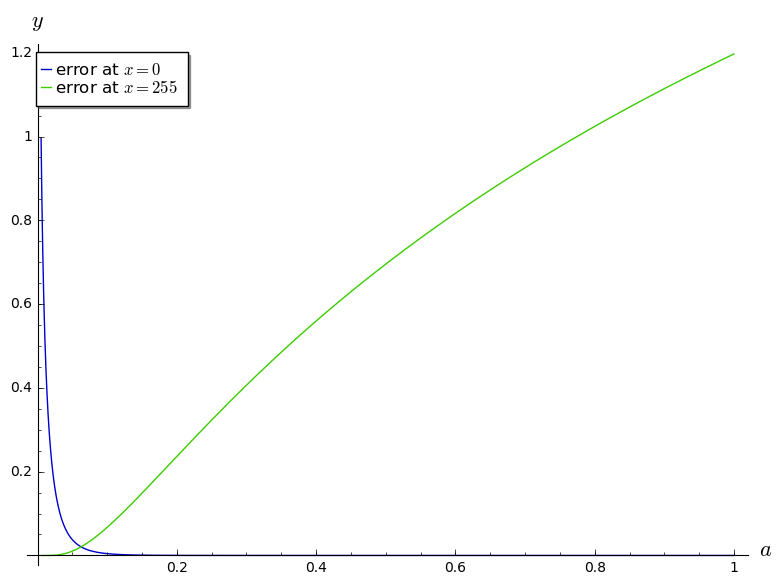
\includegraphics[width=.9\linewidth]{figures/endpoint_plot.png}
		\caption{Graphs of $A(x,\alpha)$ at $x=0$ and $x=255$.}
		\label{fig:endpoint_plot}
\end{figure}
We then consider the function $A(x,1/16)$, shown in figure \ref{fig:single_alpha_plot}.
It was determined numerically using SageMath 8.3 that the local maxima of $A(x,1/16)$ on the interval occur at $x=0$ and $x=255$. Since a scaling factor other than $alpha=1/16$ yields a higher absolute error at either $x=0$ or $x=255$, as seen in figure \ref{fig:endpoint_plot}, it follows that a scaling factor of $\alpha = 1/16$ minimizes the maximum absolute error of the scaled approximation for $\log{(1+x)}$, within the range $x \in [0, 255]$.
\begin{figure}[!ht]
		\centering
		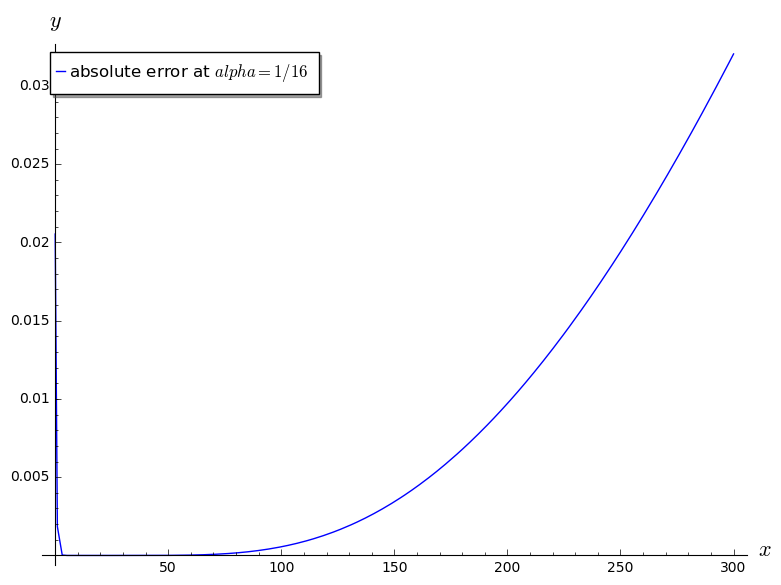
\includegraphics[width=.9\linewidth]{figures/single_alpha_plot.png}
		\caption{Graph of $A(x,1/16)$, the absolute error of the approximation in equation \ref{eq:optimal_log_approximation} given a scaling factor of $\alpha=1/16$.}
		\label{fig:single_alpha_plot}
\end{figure}

We have shown how we can adapt Khattri's approximation to allow for privacy-preserving logarithm computation over a larger interval. We note we only require the quadrature approach if series representations of the desired function are not suitable for privacy-preserving calculation using the floating-point arithmetic supported by the Paillier cryptosystem.

As a concrete example, evaluating partial sums of the series representation for the exponential function
\begin{align*}
	e^x = \sum_{n=0}^{\infty}{\frac{x^n}{n!}}
\end{align*}
is a valid approach for privacy-preserving computation, as this series converges for all $x$.
